% Options for packages loaded elsewhere
\PassOptionsToPackage{unicode}{hyperref}
\PassOptionsToPackage{hyphens}{url}
%
\documentclass[
  12pt,
]{article}
\usepackage{amsmath,amssymb}
\usepackage{lmodern}
\usepackage{ifxetex,ifluatex}
\ifnum 0\ifxetex 1\fi\ifluatex 1\fi=0 % if pdftex
  \usepackage[T1]{fontenc}
  \usepackage[utf8]{inputenc}
  \usepackage{textcomp} % provide euro and other symbols
\else % if luatex or xetex
  \usepackage{unicode-math}
  \defaultfontfeatures{Scale=MatchLowercase}
  \defaultfontfeatures[\rmfamily]{Ligatures=TeX,Scale=1}
\fi
% Use upquote if available, for straight quotes in verbatim environments
\IfFileExists{upquote.sty}{\usepackage{upquote}}{}
\IfFileExists{microtype.sty}{% use microtype if available
  \usepackage[]{microtype}
  \UseMicrotypeSet[protrusion]{basicmath} % disable protrusion for tt fonts
}{}
\makeatletter
\@ifundefined{KOMAClassName}{% if non-KOMA class
  \IfFileExists{parskip.sty}{%
    \usepackage{parskip}
  }{% else
    \setlength{\parindent}{0pt}
    \setlength{\parskip}{6pt plus 2pt minus 1pt}}
}{% if KOMA class
  \KOMAoptions{parskip=half}}
\makeatother
\usepackage{xcolor}
\IfFileExists{xurl.sty}{\usepackage{xurl}}{} % add URL line breaks if available
\IfFileExists{bookmark.sty}{\usepackage{bookmark}}{\usepackage{hyperref}}
\hypersetup{
  pdftitle={Ticketing and Turnout: The Participatory Consequences of Low-Level Police Contact},
  hidelinks,
  pdfcreator={LaTeX via pandoc}}
\urlstyle{same} % disable monospaced font for URLs
\usepackage[margin=1in]{geometry}
\usepackage{longtable,booktabs,array}
\usepackage{calc} % for calculating minipage widths
% Correct order of tables after \paragraph or \subparagraph
\usepackage{etoolbox}
\makeatletter
\patchcmd\longtable{\par}{\if@noskipsec\mbox{}\fi\par}{}{}
\makeatother
% Allow footnotes in longtable head/foot
\IfFileExists{footnotehyper.sty}{\usepackage{footnotehyper}}{\usepackage{footnote}}
\makesavenoteenv{longtable}
\usepackage{graphicx}
\makeatletter
\def\maxwidth{\ifdim\Gin@nat@width>\linewidth\linewidth\else\Gin@nat@width\fi}
\def\maxheight{\ifdim\Gin@nat@height>\textheight\textheight\else\Gin@nat@height\fi}
\makeatother
% Scale images if necessary, so that they will not overflow the page
% margins by default, and it is still possible to overwrite the defaults
% using explicit options in \includegraphics[width, height, ...]{}
\setkeys{Gin}{width=\maxwidth,height=\maxheight,keepaspectratio}
% Set default figure placement to htbp
\makeatletter
\def\fps@figure{htbp}
\makeatother
\setlength{\emergencystretch}{3em} % prevent overfull lines
\providecommand{\tightlist}{%
  \setlength{\itemsep}{0pt}\setlength{\parskip}{0pt}}
\setcounter{secnumdepth}{5}
\usepackage{rotating}
\usepackage{setspace}
\usepackage{booktabs}
\usepackage{longtable}
\usepackage{array}
\usepackage{multirow}
\usepackage{wrapfig}
\usepackage{float}
\usepackage{colortbl}
\usepackage{pdflscape}
\usepackage{tabu}
\usepackage{threeparttable}
\usepackage{threeparttablex}
\usepackage[normalem]{ulem}
\usepackage{makecell}
\usepackage{xcolor}
\ifluatex
  \usepackage{selnolig}  % disable illegal ligatures
\fi
\newlength{\cslhangindent}
\setlength{\cslhangindent}{1.5em}
\newlength{\csllabelwidth}
\setlength{\csllabelwidth}{3em}
\newenvironment{CSLReferences}[2] % #1 hanging-ident, #2 entry spacing
 {% don't indent paragraphs
  \setlength{\parindent}{0pt}
  % turn on hanging indent if param 1 is 1
  \ifodd #1 \everypar{\setlength{\hangindent}{\cslhangindent}}\ignorespaces\fi
  % set entry spacing
  \ifnum #2 > 0
  \setlength{\parskip}{#2\baselineskip}
  \fi
 }%
 {}
\usepackage{calc}
\newcommand{\CSLBlock}[1]{#1\hfill\break}
\newcommand{\CSLLeftMargin}[1]{\parbox[t]{\csllabelwidth}{#1}}
\newcommand{\CSLRightInline}[1]{\parbox[t]{\linewidth - \csllabelwidth}{#1}\break}
\newcommand{\CSLIndent}[1]{\hspace{\cslhangindent}#1}

\title{Ticketing and Turnout: The Participatory Consequences of Low-Level Police Contact}
\author{}
\date{\vspace{-2.5em}February 22, 2022}

\begin{document}
\maketitle
\begin{abstract}
The American criminal legal system is an important site of political socialization: scholars have shown that criminal legal contact reduces turnout, and that criminalization pushes people away from public institutions more broadly. Despite this burgeoning literature, few analyses directly investigate the causal effect of \emph{lower-level} police contact on voter turnout. We use two approaches to do so: we leverage both individual-level administrative ticketing data from Hillsborough County, Florida, and responses to the American National Election Studies. We estimate that a traffic stop decreases an individual's likelihood of voting by 1.7 percentage points, but depressive effects are smaller for Black residents. The survey data, however, show that Black people who report that they or a family member were recently stopped by police are \emph{more} likely to vote than those who reported no such contact. Taken together, our results indicate that low-level contact with police may have participatory consequences.

\hfill\break

\textbf{Keywords}: voting, policing, race, punishment, political participation
\end{abstract}

\pagenumbering{gobble}
\pagebreak

\pagenumbering{arabic}
\doublespacing

\hypertarget{introduction}{%
\section*{Introduction}\label{introduction}}
\addcontentsline{toc}{section}{Introduction}

Fines and fees are increasingly recognized as a form of racist revenue extraction connected to marginalized communities' alienation from government (\protect\hyperlink{ref-Sanders2017}{Sanders and Conarck 2017}; \protect\hyperlink{ref-McCoy2015}{McCoy 2015}; \protect\hyperlink{ref-Shaer2019}{Shaer 2019}). After Michael Brown was killed by the Ferguson Police Department in 2014, a US Department of Justice investigation into the city's police and courts demonstrated that the municipality was engaged in a practice that advocates now refer to as ``policing for profit.'' The city's reliance on fines and fees to fund government functions grew from 13 to 23 percent of the total budget between fiscal years 2012 and 2015. From 2012 to 2014, the Department of Justice found that 85 percent of vehicle stops, 90 percent of citations, and 93 percent of arrests targeted Black people. By contrast, just two-thirds of Ferguson's residents are Black (\protect\hyperlink{ref-UnitedStatesDepartmentofJusticeCivilRightsDivision2015}{United States Department of Justice Civil Rights Division 2015}).

It wasn't just a Ferguson problem, or even a Missouri problem. American cities' reliance on fines and fees revenue increased significantly following the 2008 recession---as local tax revenues dropped and tax increases became less politically viable, jurisdictions increased the amounts of fines and fees and imposed them more frequently in order to fund government services (\protect\hyperlink{ref-Singla2020}{Singla, Kirschner, and Stone 2020}; \protect\hyperlink{ref-Harris2017}{A. Harris et al. 2017}; \protect\hyperlink{ref-Harris2020}{A. P. Harris, Ash, and Fagan 2020}).

Although scholars have examined the collateral consequences of this increased reliance on fines and fees (\protect\hyperlink{ref-Sances2017}{Sances and You 2017}; \protect\hyperlink{ref-Pacewicz2020}{Pacewicz and Robinson 2020}), comparatively few have explored the moment during which such revenue-raising actually occurs: namely, in the individual interactions between residents and the police via the issuance of a ticket. This ``moment'' of low-level contact has also been relatively understudied by scholars investigating the participatory consequences of contact with the criminal legal system. Work exploring how criminalization directly and indirectly influences political participation has exploded in recent years. Scholars have found that criminal legal contact (i.e.~arrest, conviction, incarceration) consistently discourages voting (\protect\hyperlink{ref-Weaver2010}{Weaver and Lerman 2010}; \protect\hyperlink{ref-Burch2011}{Burch 2011}; \protect\hyperlink{ref-White2019a}{White 2019b}). Such work has largely focused on the effects of highly disruptive contact with the criminal legal system such as incarceration and felony convictions (\protect\hyperlink{ref-Burch2014}{Burch 2014}; \protect\hyperlink{ref-Lee2014}{Lee, Porter, and Comfort 2014}). While ticketing involves potentially negative interactions with the state, it does not necessarily carry the disruptive consequences of a felony conviction and might thus politicize Americans in unique ways. Building on recent theoretical work from \protect\hyperlink{ref-Walker2020a}{Walker} (\protect\hyperlink{ref-Walker2020a}{2020b}), this paper theorizes how local police practices affect voting behavior among ticketed individuals and provides precisely estimated evidence of a causal effect.

Our project represents the first use of individual-level administrative data to identify the causal effect of traffic stops on voter behavior. The use of administrative data marks an important step forward in our understanding of how low-level contact with the criminal legal system structures political participation. Past work looking at the individual-level effects of low-level contact has relied on survey or qualitative data (e.g. \protect\hyperlink{ref-Walker2014}{Walker 2014}; \protect\hyperlink{ref-Weaver2010}{Weaver and Lerman 2010}). Existing research allows for the testing of specific psychological mechanisms and personal interpretations of criminal legal contact, but does not allow us to generalize more broadly. As Weaver and Lerman (\protect\hyperlink{ref-Weaver2010}{2010}: 821) note, it may also introduce measurement bias. Our analysis investigates actual voting behavior following actual ticketing events, not reported voting behavior or reported exposure to a traffic stop. The administrative data therefore allow us both to sidestep reporting error and to observe the behavior of a quarter-million individuals stopped over a 6 year period---a far larger pool than even the most robust surveys.

We use individual-level traffic stop data from Hillsborough County, Florida, to identify the turnout patterns of voters who were stopped between the 2012 and 2018 elections. By matching individual voters who were stopped to similar voters who were stopped at later points and running a difference-in-differences model, we estimate the causal effect of these stops on turnout. This borrows from the logic of regression discontinuities in time: conditional on observable characteristics \emph{and} unobservable factors associated with being ticketed, the timing of the ticket on either side of election day is essentially as-if random. We find that being stopped reduces the chance that an individual will turn out in the subsequent election, but that this effect is smaller for Black voters.

To test the generalizability of our findings in Hillsborough County, we conduct a novel analysis of 2020 national survey data regarding voters' experience with police stops. We find that Black respondents who reported personal or proximal experience with police stops in the last 12 months are more likely to vote than Black people who did not, while we find no statistically significant relationship between stops and voting among non-Black respondents. While the survey data present some drawbacks relative to the individual-level administrative data, their national scope provides helpful corroboration for the unique turnout effects of traffic stops for Black Americans observed in Hillsborough County.

We demonstrate that police ticketing practices---the most widespread form of police contact in America---substantially reduce the turnout of non-Black American voters, but have a unique effect on Black voter turnout. Our findings complicate existing theories of how criminalization politically socializes Americans, and Black Americans in particular (\protect\hyperlink{ref-Weaver2010}{Weaver and Lerman 2010}). Additionally, while many forms of criminalization have been found to contribute to a well-documented subjective experience of alienation or group-level exclusion among Black Americans (\protect\hyperlink{ref-Bell2017}{Bell 2017}; \protect\hyperlink{ref-Stuart2016}{Stuart 2016}; \protect\hyperlink{ref-Desmond2016}{Desmond, Papachristos, and Kirk 2016}, \protect\hyperlink{ref-Desmond2020}{2020}; \protect\hyperlink{ref-Zoorob2020}{Zoorob 2020}; \protect\hyperlink{ref-Ang2021}{Ang et al. 2021}), our contribution emphasizes the need for further research regarding how different forms of criminalization affect group-level perceptions of government and resultant political behaviors. Our findings are relevant for interdisciplinary scholars of crime, race, politics, municipal finance, and policing.

\hypertarget{criminal-legal-system-and-citizen-identity}{%
\section*{Criminal Legal System and Citizen Identity}\label{criminal-legal-system-and-citizen-identity}}
\addcontentsline{toc}{section}{Criminal Legal System and Citizen Identity}

In recent years, scholars have paid more attention to the political implications of the American criminal legal system. Evolving in part out of a literature focused on street-level bureaucrats, researchers across the social sciences are asking how daily interactions with agents of the carceral state shape Americans' relationships to themselves, their communities, and their state. As \protect\hyperlink{ref-Soss2017}{Soss and Weaver} (\protect\hyperlink{ref-Soss2017}{2017}) argues, this ``second face'' of the state---``the activities of governing institutions and officials that exercise social control and encompass various modes of coercion, containment, repression, surveillance, regulation, predation, discipline, and violence'' (567)---is the primary way through which many class-race subjugated communities develop their political knowledge. ``{[}I{]}nterviewees have looked, not to City Hall, Congress, or political parties,'' they write, ``but rather to their direct experiences with police, jails and prisons, welfare offices, courts, and reentry agencies as they sought to ground their explanations of how government works, what political life is like for them, and how they understand their own political identities'' (\protect\hyperlink{ref-Soss2017}{Soss and Weaver 2017, 574}).

Recent work has explored the production of this political knowledge in increasingly sophisticated ways, using both qualitative and quantitative approaches. \protect\hyperlink{ref-Lerman2014}{Lerman and Weaver} (\protect\hyperlink{ref-Lerman2014}{2014})'s pathbreaking book \emph{Arresting Citizenship} set the table for future research. Their project combined extensive interviews of individuals living in areas closely monitored by the criminal legal system with novel survey data to probe the political consequences of what they term the ``carceral state.'' Their work indicates that citizens nearly uniformly react negatively to police and carceral supervision---from low-level interactions to lengthy periods of incarceration, Americans subjected to the second face of the state apparently withdraw from political participation. They find that trust in government and willingness to vote decrease as individuals progress through increasingly intense levels of criminal legal contact (questioned by police, arrested, convicted, incarcerated) (\protect\hyperlink{ref-Weaver2010}{Weaver and Lerman 2010}). New evidence related to ticketing and legal estrangement has recently emerged: in a survey of residents in three Georgia cities that rely heavily on fines and fees revenue, residents who were ticketed reported lower levels of trust in police and government compared to residents who were not ticketed (\protect\hyperlink{ref-CarpenterII2019}{Carpenter II, Sweetland, and McDonald 2019}).

Sarah Brayne (\protect\hyperlink{ref-Brayne2014}{2014}) found related results in her analysis of survey data. As the intensity of criminal legal contact escalates , people subjected to criminalization are increasingly likely to avoid institutions that they perceive as surveilling, such as financial or educational institutions. She calls this phenomenon ``system avoidance,'' and while her analysis did not specifically assess voting behavior, her findings demonstrate how criminal legal contact can discourage Americans' participation in public institutions as well as how the effect may vary alongside the intensity of criminal legal intervention. Similarly, \protect\hyperlink{ref-Remster2018a}{Remster and Kramer} (\protect\hyperlink{ref-Remster2018a}{2018}) finds that men who return home from prison are more likely to avoid contact with their childrens' schools. Vesla Weaver and colleagues describe this form of self-preserving withdrawal from public institutions as a ``strategic retreat'' (\protect\hyperlink{ref-Weaver2020}{Weaver, Prowse, and Piston 2020}).

These findings can be situated in a process that sociologist Monica Bell calls ``legal estrangement,'' which captures those perceptions and cultural attitudes (``legal cynicism'') as well as the historical-structural conditions that produced them (\protect\hyperlink{ref-Bell2017}{Bell 2017}). Research on legal cynicism has found that public perceptions of abusive police practices can reduce willingness to report crimes or cooperate with law enforcement (\protect\hyperlink{ref-Tyler2014}{Tyler, Fagan, and Geller 2014}). The ``hidden curriculum'' (\protect\hyperlink{ref-Justice2014}{Justice and Meares 2014}; \protect\hyperlink{ref-Meares2017}{Meares 2017}) of the criminal legal system teaches Americans about their identities as citizens---even parts of their identities that have little to do with policing or incarceration.

\hypertarget{administrative-data-and-the-causal-effects-of-criminalization}{%
\section*{Administrative Data and the Causal Effects of Criminalization}\label{administrative-data-and-the-causal-effects-of-criminalization}}
\addcontentsline{toc}{section}{Administrative Data and the Causal Effects of Criminalization}

Many scholars have turned to administrative data in recent years to explore the actual effects of contact with the criminal legal system on political participation in the voting booth. To be sure, administrative data have limitations: they are not ideally suited to probe the psychological, social, relational, and other mechanisms leading some citizens to vote and others to abstain. These limitations, however, are balanced by offering researchers precise estimates of actual---and not just reported---turnout.

Traci Burch (\protect\hyperlink{ref-Burch2011}{2011}) was among the earliest scholars to match voter-file records with records detailing citizens' contact with the criminal legal system. Her work complicated a previously dominant theory postulating that the turnout and party registration of formerly incarcerated individuals was largely driven by their sociodemographic characteristics but not their formal conviction or supervision (see, for instance, \protect\hyperlink{ref-Uggen2002}{Uggen and Manza 2002}). She argues that citizens who are convicted of felony offenses are less likely to vote, and less likely to register with a party, than citizens with similar sociodemographic characteristics without such a conviction.

Other scholars have similarly matched corrections records with registered voter files to explore the effect of contact with the second face of the state. \protect\hyperlink{ref-White2019a}{White} (\protect\hyperlink{ref-White2019a}{2019b}) finds that short periods of incarceration reduce Black, but not white, turnout. \protect\hyperlink{ref-Gerber2017}{Gerber et al.} (\protect\hyperlink{ref-Gerber2017}{2017}) similarly finds relatively small effects of incarceration on turnout. Meredith and Morse (\protect\hyperlink{ref-Meredith2014}{2014}, \protect\hyperlink{ref-Meredith2015}{2015}) and \protect\hyperlink{ref-Gerber2015}{Gerber et al.} (\protect\hyperlink{ref-Gerber2015}{2015}) explore the turnout effect of notifying formerly incarcerated citizens of the legal restoration of their voting rights, with mixed results, while \protect\hyperlink{ref-Morris2021a}{Morris} (\protect\hyperlink{ref-Morris2021a}{2021a}) shows that restoring voting rights to individuals while they are still on parole increases post-supervision turnout. Other work has explored the ``spillover'' effects of such contact, finding that the political behavior of family members (\protect\hyperlink{ref-White2019}{White 2019a}) and neighbors (\protect\hyperlink{ref-Burch2014}{Burch 2014}; \protect\hyperlink{ref-Morris2020}{Morris 2020}) can be influenced by indirect contact with incarceration. \protect\hyperlink{ref-Morris2021}{Morris} (\protect\hyperlink{ref-Morris2021}{2021b}) argues that these effects are durable, showing that citizens whose household members had been to prison were not disproportionately mobilized by a ballot initiative promising to end felony disenfranchisement.

This burgeoning literature using administrative data has given scholars far greater insight into the participatory consequences of American incarceration. It is, however, virtually silent on the effects of \emph{lower level} contact with the criminal legal system. Far more Americans have low-level contact with the police than will ever spend a night behind bars: just under 20 million Americans experience a traffic stop each year, whereas approximately five million Americans are arrested and jailed each year (\protect\hyperlink{ref-Harrell2020}{Harrell and Davis 2020}; \protect\hyperlink{ref-Jones2019}{Jones and Sawyer 2019}). Despite the fact that so many more citizens are subjected to traffic stops, we know comparatively little about its political ramifications, a lack that is particularly glaring given how much we have learned in recent years about higher-level contact.

The one project that has used administrative data to explore the political implications of low-level police contact is \protect\hyperlink{ref-Laniyonu2019}{Laniyonu} (\protect\hyperlink{ref-Laniyonu2019}{2019}), which explores the effects of the Stop, Question, and Frisk (SQF) program in New York City. \protect\hyperlink{ref-Laniyonu2019}{Laniyonu} (\protect\hyperlink{ref-Laniyonu2019}{2019})'s causal estimates rely on a cross-sectional matching model to compare voter turnout in precincts with \emph{high} SQF activity to turnout in precincts with similar sociodemographic characteristics but \emph{low} SQF activity, supplemented with cross-sectional analyses of all precincts in the city. His results paint a complicated picture: his causal estimates find that high levels of SQF increased turnout in the 2008 presidential election, but decreased it in the 2010 midterms. While \protect\hyperlink{ref-Laniyonu2019}{Laniyonu} (\protect\hyperlink{ref-Laniyonu2019}{2019}) marks an important step forward in the investigation of the consequences of policing for political behavior, it faces certain data and methodological limitations. Because the SQF data does not include identifying information about the individuals stopped, he cannot explore the turnout of New Yorkers who were actually subjected to SQF. Thus, as he notes in the conclusion, ``the ability of the analysis to make causal claims is limited'' (554) by the cross-sectional matching approach.

In this project, we seek to extend our understanding of the political consequences of routine contact with the state's second face. Combining an individual-level administrative panel dataset with national survey data gives us new insight into how traffic stops can shape citizens' engagement with their democracy.

\hypertarget{how-police-stops-might-structure-turnout}{%
\section*{How Police Stops Might Structure Turnout}\label{how-police-stops-might-structure-turnout}}
\addcontentsline{toc}{section}{How Police Stops Might Structure Turnout}

Much of the existing work on the turnout consequences of the criminal legal system points to a process of political learning or political socialization. \protect\hyperlink{ref-Lerman2014}{Lerman and Weaver} (\protect\hyperlink{ref-Lerman2014}{2014}) finds that individuals in highly surveilled neighborhoods learn that the government does not care about them, and is uninterested in soliciting their participation. They note that more than half of individuals stopped by the police report agreeing with the statement ``the leaders in government care very little about people like me,'' compared with just a third of respondents with no police contact (150). The numbers, however, were far higher for individuals convicted of a crime, of whom three-quarters agreed with the statement. Learning about the criminal legal system takes place over a long period of time. Could isolated police stops that neither require sustained contact with the criminal legal system nor (generally) impose punishments as severe as incarceration politically socialize Americans to the same degree as incarceration?

On one hand, it might seem unlikely that a single stop would produce much new knowledge about the state. For many Americans, a traffic stop amounts to little more than a slap on the wrist. To be sure, fines and fees can wreak havoc on the lives of some drivers. If a ticket leads to a suspended driver's license, the initial stop can snowball into a much bigger life event that could jeopardize employment, or lead to shorter stints of incarceration for individuals apprehended driving on a suspended license. Searches conducted during traffic stops may also lead to arrest or incarceration if a police officer finds contraband in the vehicle. These comparatively less frequent cases might have consequences more akin to those associated with a brief period of incarceration that can also threaten employment. Nevertheless, the average traffic stop is certainly less disruptive than the average period of incarceration, perhaps producing less political knowledge and therefore impacting turnout less.

On the other hand, a far larger set of Americans are stopped by the police than sent to jail or prison each year. According to the American National Election Study, a nationally-representative survey we use later in this study, the incomes and education levels for individuals stopped by the police are meaningfully higher than for individuals who report ever having been arrested. Motorists stopped by police are apparently systematically different compared to people who experience incarceration. Traffic stops might thus be the primary way some of these Americans learn about the criminal legal system. If these Americans have not already ``learned'' about the system from their neighborhoods or family members, the political consequences of such newly gleaned knowledge might be large.

Traffic stops might provide early insights about the criminal legal system even for Americans who live in more heavily-policed areas. As \protect\hyperlink{ref-Gerber2017}{Gerber et al.} (\protect\hyperlink{ref-Gerber2017}{2017}) notes in their study arguing that the participatory consequences of incarceration might be small, incarceration ``is an outcome that often follows a long series of interactions with the criminal justice system'' (1145). In other words, much of what the criminal legal system ``teaches'' might have already been learned by the time an individual is sent to prison. Someone who is stopped by the police, however, might have had fewer negative interactions with the state. Put differently, stopped individuals might have more to learn than incarcerated individuals with a long history of police contact, resulting in higher turnout effects.

\hypertarget{potential-for-racially-disparate-effects}{%
\section*{Potential for Racially Disparate Effects}\label{potential-for-racially-disparate-effects}}
\addcontentsline{toc}{section}{Potential for Racially Disparate Effects}

The potential for more ``learning'' from a police stop seems especially salient for Black Americans, particularly in recent years. National news over the 2010s was filled with the names of Black Americans who were killed during routine police stops. The Black Lives Matter movement gained national attention in the aftermath of the Ferguson uprising, an uprising sparked by the police killing of Michael Brown but also fueled by that city's racial discriminatory ticketing practices. In the fall of 2021, \emph{The New York Times} ran an extensive report exploring police killings that occur during traffic stops, providing more proof of their racially disparate nature (\protect\hyperlink{ref-Levenson2021}{Levenson 2021}).

We expect that the participatory consequences of such a stop will be different for Black than non-Black Americans. First, traffic stops differ in meaningful ways for Black and non-Black Americans. As \protect\hyperlink{ref-Baumgartner2018}{Baumgartner, Epp, and Shoub} (\protect\hyperlink{ref-Baumgartner2018}{2018}) notes, Black Americans are more likely than whites to receive both ``light'' (i.e., a warning without a ticked) \emph{and} ``severe'' (i.e., arrest) outcomes from a traffic stop. Although this may seem paradoxical at first, the authors explain: ``while many might rejoice in getting a warning rather than a ticket, the racial differences consistently apparent in the data suggest another interpretation for black drivers: even the officer recognized that there was no infraction'' {[}88{]}. Black drivers are also more likely to be searched and arrested, but less likely to be found with contraband (\protect\hyperlink{ref-Baumgartner2018}{Baumgartner, Epp, and Shoub 2018}). Similarly, \protect\hyperlink{ref-Epp2014}{Epp, Maynard-Moody, and Haider-Markel} (\protect\hyperlink{ref-Epp2014}{2014}) argues that traffic stops are particularly instructive for Black Americans, as pretextual traffic stops politically socialize Black voters to the specific context of discriminatory police ticketing.

The politicization of a police stop can occur differently for Black Americans through other avenues as well. The BLM movement has raised the salience of racially disparate policing across the country, as have the tragic stories of individuals like Philando Castile who was killed during a police stop. Routine interactions with the police are also more likely to turn deadly for Black Americans than for others (\protect\hyperlink{ref-Levenson2021}{Levenson 2021}). Thus, even if an individual police stop for a Black American is relatively unremarkable on its own, the background context that the interaction \emph{could} have turned deadly is likely to result in some level of trauma for Black drivers. Recent work from Hannah Walker (\protect\hyperlink{ref-Walker2020}{2020a}, \protect\hyperlink{ref-Walker2020a}{2020b}) argues that this could lead to a \emph{mobilizing} effect, if stopped drivers understand their contact with the criminal legal system in the context of a narrative of racial injustice, such contact can actually mobilize. She explains: ``experiences with punitive policies are subject to interpretation and, when understood through narratives of injustice, lead to wholly different participation outcomes than we usually predict'' (\protect\hyperlink{ref-Walker2020}{Walker 2020a, 132}). While she finds that this sense of injustice is especially likely to increase political participation in non-voting ways (such as attending a protest or signing a petition), the logic could extend to electoral participation as well given a relevant electoral context, strong injustice narrative, or relatively weak contact with the criminal legal system.

Given that police stops are more likely to be traumatic for Black motorists (because traffic stops come with a threat of escalation into racialized police violence, because they received harsher punishments, \emph{or} because the stop itself was discriminatory) \emph{and} that there exists a framework available for translating negative experiences with the criminal legal system into political action, we expect police stops to have unique participatory consequences for Black Americans.

At the same time, the average Black American already knows far more about the criminal legal system due to the extreme racial disparities in policing and incarceration. As one 2015 study observed, 44\% of Black women (and 32\% of Black men) have a family member in prison. These numbers compare with just 12\% and 6\% for white women and men, respectively (\protect\hyperlink{ref-Lee2015}{Lee et al. 2015}). Black Americans' disproportionate contact with the criminal legal system is a firmly established fact at this point. This greater baseline exposure could mean that Black Americans have less to ``learn'' from a marginal police stop, resulting in smaller turnout effects.

\hypertarget{data-and-design}{%
\section*{Data and Design}\label{data-and-design}}
\addcontentsline{toc}{section}{Data and Design}

We leverage two distinct approaches to ask whether police traffic stops affect voter turnout, and whether these effects are unique for Black Americans.

Each approach offers advantages and drawbacks. Our individual-level analysis in Hillsborough County exploits unusually detailed public data, which allows for a precise causal analysis that cannot be conducted in counties that do not provide ticketing records with personally identifiable information or states that do not include self-reported race data in the voter file. The empirical estimand is the voter turnout gap between Hillsborough County residents who have recently been ticketed and residents who will be ticketed in a future period, conditional on similar turnout in past elections and similar demographic characteristics. In isolation, however, results from one county may not be generalizable to other U.S. counties.

Data from the 2020 American National Election Studies allow us to observe how tickets and arrests differentially influence voting behavior at the individual level among a nationally representative sample, but survey data analysis is subject to the vulnerabilities detailed in our introduction (e.g.~measurement bias). Nevertheless, it provides important national insight into the phenomena we observe locally in Hillsborough County.

Taken together, these approaches advance our understanding of the political consequences of the most routine types of contact with the criminal legal system.

\hypertarget{individual-level-causal-effects-of-traffic-stops}{%
\subsection*{Individual-Level Causal Effects of Traffic Stops}\label{individual-level-causal-effects-of-traffic-stops}}
\addcontentsline{toc}{subsection}{Individual-Level Causal Effects of Traffic Stops}

First, we turn to individual-level data from Hillsborough County, Florida (home to Tampa).
Hillsborough County makes a unique set of data publicly available. The county clerk makes information available about every traffic stop in the county going back to 2003. This data includes the name and date of birth of the individual stopped; the date of the offense; the amount the individual paid for a ticket; and other information.

To identify ticketed voters, we match the first and last names and dates of birth from the stop data against the Hillsborough County registered voter file. \protect\hyperlink{ref-Meredith2014}{Meredith and Morse} (\protect\hyperlink{ref-Meredith2014}{2014}) develops a test for assessing the prevalence of false-positives in administrative record matching. We present the results of that test in section 1 of the Supplementary Information (SI). We likely have a false-positive match of around 0.03 percent, a figure we consider too low to impact our results meaningfully.

Using a single post-treatment snapshot of the voter file can result in conditioning on a post-treatment status (see \protect\hyperlink{ref-Nyhan2017}{Nyhan, Skovron, and Titiunik 2017}). Instead, we collect snapshots of the voter file following each even-year general election between 2012 and 2018.\footnote{Because such frequent snapshots are not available from L2, we here use the registered voter file made freely available by the state of Florida.} We thus observe virtually all individuals who were registered to vote at any time during our period of study. Unique voter identification numbers allow us to avoid double-counting voters who are registered in multiple snapshots. We retain each voter's earliest record, and geocode voters to their home census block groups. Because we argue that police contact is the driving force behind any turnout effect, we remove tickets issued by red-light cameras.

By matching the police stop and voter records, we identify all voters who were stopped between the 2012 and 2020 general elections (voters stopped between 2018 and 2020 elections serve only as controls). We collect self-reported information regarding the race of each voter from Florida's public voter file rather than the police stop data. Voters are considered ``treated'' in the general election following their stop. Treated voters are then matched to a control voter using a nearest-neighbor approach, with a genetic algorithm used to determine the best weight for each characteristic (\protect\hyperlink{ref-Sekhon2011}{Sekhon 2011}). Control voters are individuals who are stopped in the two years following the post-treatment election of the treated voters. Put differently, if a voter is stopped between 2012 and 2014, their control voter must be an individual stopped between the 2014 and 2016 elections. A voter cannot both be a treated and control voter for the same election; therefore, someone stopped between the 2012 and 2014 elections and again between the 2014 and 2016 elections cannot serve as a control for anyone stopped between 2012 and 2014. We limit the target population to voters who are stopped at some point in order to account for unobserved characteristics that motivate people who are stopped at some point to turn out at higher rates than people who are never stopped.

We match voters on individual-level characteristics (race / ethnicity; gender; party affiliation; age; number of traffic stops prior to the treatment period) and block group-level characteristics from the 2012 5-year ACS estimates (median income; share of the population with some college; unemployment rate). We match exactly on the type of ticket (civil / criminal infraction; whether they paid a fine; whether they were stopped by the Tampa Police Department) to ensure that treated and control voters receive the same treatment. Finally, we match treated and control voters on their turnout in the three pre-treatment elections.

We assume that after controlling for observable characteristics, past turnout, \emph{and} the unobservable characteristics associated with experiencing a traffic stop, the timing of the stop is effectively random. This is conceptually similar to the regression discontinuity in time framework, and we assume that any turnout difference between the treated voters and their controls is the causal effect of a police stop on turnout. Our overall turnout effects are robust to much weaker assumptions: in section 2 of the SI, we demonstrate that our overall turnout results hold even when we force voters stopped shortly before the election to match to voters stopped shortly afterwards.

Our analytical design thus incorporates two different causal approaches in order to improve the credibility of our identification assumptions. Leveraging pre-treatment turnout allows us to estimate a traditional difference-in-differences model, while the matching procedure improves the plausibility of the parallel trends assumption by reducing salient differences between the treated and control voters. For a more detailed discussion of how matching can improve upon traditional difference-in-difference approaches when using panel data, see \protect\hyperlink{ref-Imai2020}{Imai, Kim, and Wang} (\protect\hyperlink{ref-Imai2020}{2020}).

We then estimate the following equation:

\begin{gather}
\label{eq:1}
v_{it}=\beta_0+\beta_1Treated_{i}+\beta_2Post Treatment_{t} + \nonumber \\
\beta_3Treated_{i}\times Post Treatment_{t} + \\
\beta_4Year_{t} + \delta{Z}_{i} + \mathcal{E}_{it}. \nonumber
\end{gather}

Individual \emph{i}'s turnout (\emph{v}) in year \emph{t} is a function of the year and whether they were stopped by the police. In the equation, \emph{\(\beta\)\textsubscript{1}Treated\textsubscript{i}} measures the historical difference between treated voters and their controls. \emph{\(\beta\)\textsubscript{2}Post Treatment\textsubscript{t}} measures whether turnout increased for controls in the first election following the treated voter's stop, while \emph{\(\beta\)\textsubscript{3}Treated\textsubscript{i} × Post Treatment\textsubscript{t}} tests whether turnout changed differently for treated voters than their controls in the election following their police stop. \emph{\(\beta\)\textsubscript{3}}, then, will capture the causal effect of a police stop on voter turnout; it is the unit-specific quantity measured in our empirical estimand (\protect\hyperlink{ref-Lundberg2021}{Lundberg, Johnson, and Stewart 2021}). \emph{\(\beta\)\textsubscript{4}Year\textsubscript{t}} captures year fixed-effects depending on the timing of the police stop, and the matrix \emph{\(\delta\)Z\textsubscript{i}} contains the individual- and neighborhood-level characteristics on which the match was performed, included in some of the models.

In some models, we also interact the treatment variable with a dummy indicating whether the voter is Black to determine race-specific treatment effects.

\hypertarget{national-survey-data}{%
\subsection*{National Survey Data}\label{national-survey-data}}
\addcontentsline{toc}{subsection}{National Survey Data}

Next, we turn to the American National Election Studies 2020 Time Series data (ANES). The ANES has been fielded in every presidential election year since 1948 and is among the most widely-used tools for understanding American's political beliefs and behaviors, including their relationship with the criminal legal system (\protect\hyperlink{ref-Walker2020}{Walker 2020a}). It is weighted to be nationally representative of all American adults. In both 2016 and 2020, the ANES added new survey questions about respondent's encounters with the police and the criminal legal system. We focus in particular on two questions: \emph{During the past 12 months, were you or any of your family members stopped or questioned by a police officer, or did this not happen in the past 12 months?}, and \emph{Have you ever been arrested, or has that never happened to you?} We include the roughly 87 percent of respondents that answered both questions, giving us a sample size of 7,347 respondents, of whom just over 11\% identified as Black.

We use these survey questions to make descriptive inferences about how stops and arrests affect the voting behavior of the general population. The first descriptive estimand is the gap between the voter turnout rate of individuals who were recently stopped by the police or who have ever been arrested, and another is whether stops or arrests uniquely influence the political behavior of Black Americans. In addition to the respondent's contact with the criminal legal system, we control for age; sex; income; education; party affiliation; self-described ideology; and reported 2016 turnout.

There is an important caveat to the use of the ANES survey---namely, while the police stop question asks whether the respondent \emph{or anyone in their family} was stopped in the past year, the arrest question asks only about the individual respondent. While this may muddy the water between direct and proximal contact with the criminal legal system, we expect that the national survey data will give us some insight into the uniquely politicizing nature of police stops for Black Americans.

\hypertarget{results}{%
\section*{Results}\label{results}}
\addcontentsline{toc}{section}{Results}

As discussed above, we begin by examining whether the turnout of individuals stopped before an election was different from those stopped after the election in Hillsborough County, Florida.
We also test the relationship between police stops and turnout in the 2020 election using survey data.

\hypertarget{individual-level-results}{%
\subsection*{Individual-Level Results}\label{individual-level-results}}
\addcontentsline{toc}{subsection}{Individual-Level Results}

To observe the effect of being stopped by the police on voter participation, we now turn to our individual-level analysis in Hillsborough County, Florida. As discussed above, we match individuals who were stopped between the 2012 and 2018 elections to individuals who were stopped following the subsequent general election.\footnote{Due to computing constraints, a 5 percent random sample stratified by treatment status is used to calculate the genetic weights. The full sample is used in the actual matching process.} Matching is done with replacement and ties are not broken. This means that some treated voters have multiple controls; the regression weights are calculated to account for this possibility. In Table \ref{tab:balance} we present the results of the matching algorithm. As the table demonstrates, the selected control voters are very similar to the treated voters.

\begin{singlespace}
\input{"../temp/balance_table.tex"}
\end{singlespace}

It is worth noting that voters who were stopped between 2012 and 2020 were far more likely to be Black and male than the general electorate, and live in Census block groups with moderately lower incomes.

In Figure \ref{fig:did-1}, we plot the turnout of treated and control voters in the elections before and after the treated voter was stopped. In the top row, we present the turnout in 2008--2014 of the individuals stopped between 2012 and 2014 and their controls; the second row shows the 2010--2016 turnout for individuals stopped between 2014 and 2016 and their controls; and the third shows the treatment effect for those stopped in the 2 years prior to the 2018 midterms. Finally, in the bottom row, we present the overall turnout effects for these three elections. The first election following a treated voter's stop is denoted as \emph{t = 0} while the years in which \emph{t} is less than zero are the periods prior to the stop.

\begin{figure}[H]

{\centering 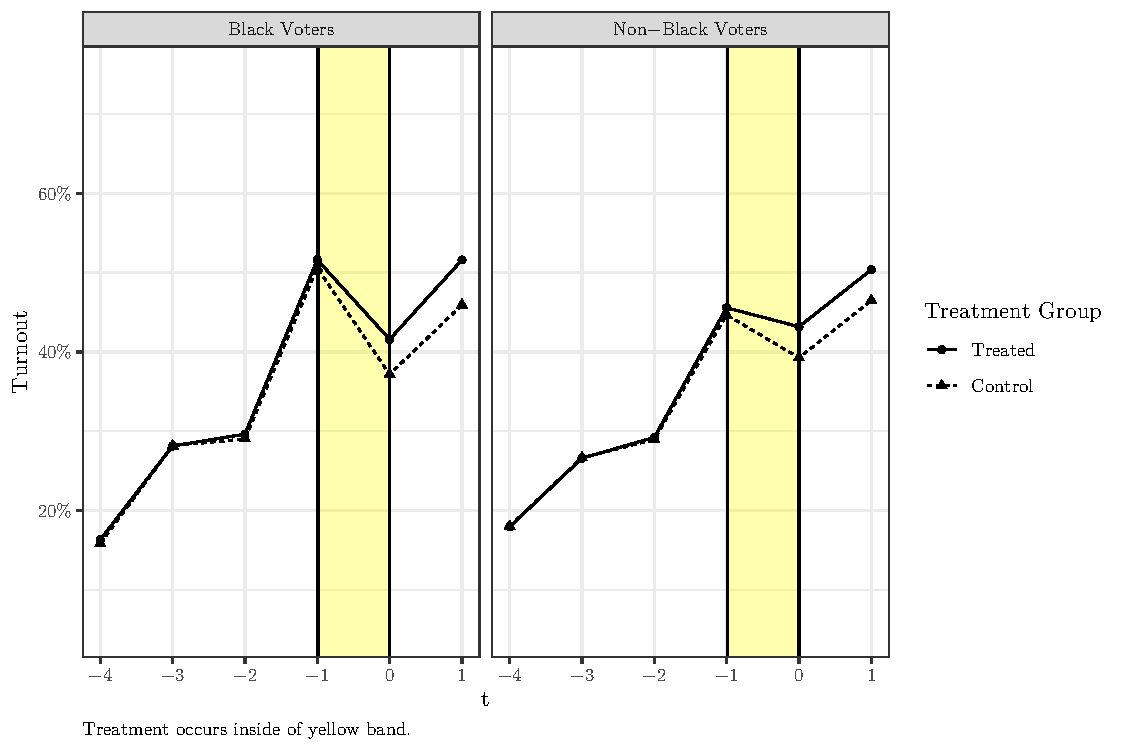
\includegraphics{draft_paper_files/figure-latex/did1-1} 

}

\caption{\label{fig:did-1}Effect of Being Ticketed on Turnout}\label{fig:did1}
\end{figure}

Figure \ref{fig:did-1} makes a number of things immediately apparent. First, we can see that for both Black and non-Black voters the pre-treatment trends are identical. This, combined with the fact that treated and control voters mirror one another in terms of other characteristics, lends credibility to the parallel trends assumption. Secondly, Figure \ref{fig:did-1} provides preliminary visual evidence of the demobilizing effects of police stops in Hillsborough County. However, as the figure also makes clear, it seems that the negative effects are concentrated in the lower-salience midterm elections; there is little evidence of turnout effects in the 2016 presidential election.

Table \ref{tab:dind-table} formalizes the final row of Figure \ref{fig:did-1} into an ordinary least squares regression (the regression tables broken out for each year and including the coefficients for the matching covariates can be found in section 3 of the SI). Models 1 and 2 show our overall causal effect, while models 3 and 4 allow for the possibility that a ticket differentially mobilizes Black voters. In models 1 and 3, we include only the treatment, timing, and race dummies, while the full set of covariates used for the matching procedure are included in models 2 and 4. The empirical estimands are \emph{Treated × Post Treatment} and \emph{Treated × Post Treatment × Black}. In models 1 and 2, the coefficient on \emph{Treated × Post Treatment} measures the overall treatment effect, and in models 3 and 4 it measures the treatment effect for non-Black voters. The coefficient on \emph{Treated × Post Treatment × Black} measures any effect for Black voters above-and-beyond the effect measured for non-Black voters.

\begin{singlespace}
\input{"../temp/small_two_matches_reg_y_overall.tex"}
\end{singlespace}

As both Figure \ref{fig:did-1} and Table \ref{tab:dind-table} make clear, traffic stops meaningfully depressed turnout. In models 1 and 2, the estimated overall treatment effect is -1.5 percentage points. In models 3 and 4, we can see that a stop was less demobilizing for Black individuals than for others---non-Black turnout was depressed by 1.7 percentage points, while the negative effect was just 1.2 points for Black individuals. Although the treatment effect is still substantively quite large for Black individuals, Hillsborough County Black voters' turnout in federal elections was not as negatively impacted by police contact as that of non-Black individuals. It is also clear that midterm turnout is more impacted by these stops---as we show in section 3 of the SI, the negative impact is statistically significant in all years for non-Black residents, but much smaller in 2016 (-0.6pp) than in 2014 (-1.9pp) or 2018 (-3.0pp),

\hypertarget{national-survey-data-1}{%
\subsection*{National Survey Data}\label{national-survey-data-1}}
\addcontentsline{toc}{subsection}{National Survey Data}

In this section we make use of the American National Election Studies 2020 Time Series Data (ANES). The first test is simple: we ask whether, after controlling for standard covariates, having personal or proximal contact with a police stop in the previous 12 months is associated with whether a respondent voted in the 2020 presidential election. We also ask whether this relationship was different for Black and non-Black respondents. Finally, we use the ANES data to reconfirm prior literature demonstrating that higher-level contact with the criminal legal system is associated with lower turnout, as these relationships could have changed in the aftermath of the widespread protests following the police murder of George Floyd in 2020.

Roughly 15 percent of non-Black respondents reported a police stop in the preceding 12 months, while the same was true for more than 22 percent of Black respondents. In Figure \ref{fig:anes} we present the results of our econometric models. In the left-hand panel, we show the predicted turnout of respondents who answered ``yes'' or ``no'' to the question \emph{During the past 12 months, were you or any of your family members stopped or questioned by a police officer, or did this not happen in the past 12 months?} The right-hand panel, meanwhile, plots these relationships for respondents who answered ``yes'' or ``no'' to the question \emph{Have you ever been arrested, or has that never happened to you?}. These are the predicted probabilities after controlling for respondents' race / ethnicity; age; party; ideology; income; education; and 2016 turnout. The full regression table can be found in section XX of the SI.

\begin{figure}[!htpb]

{\centering 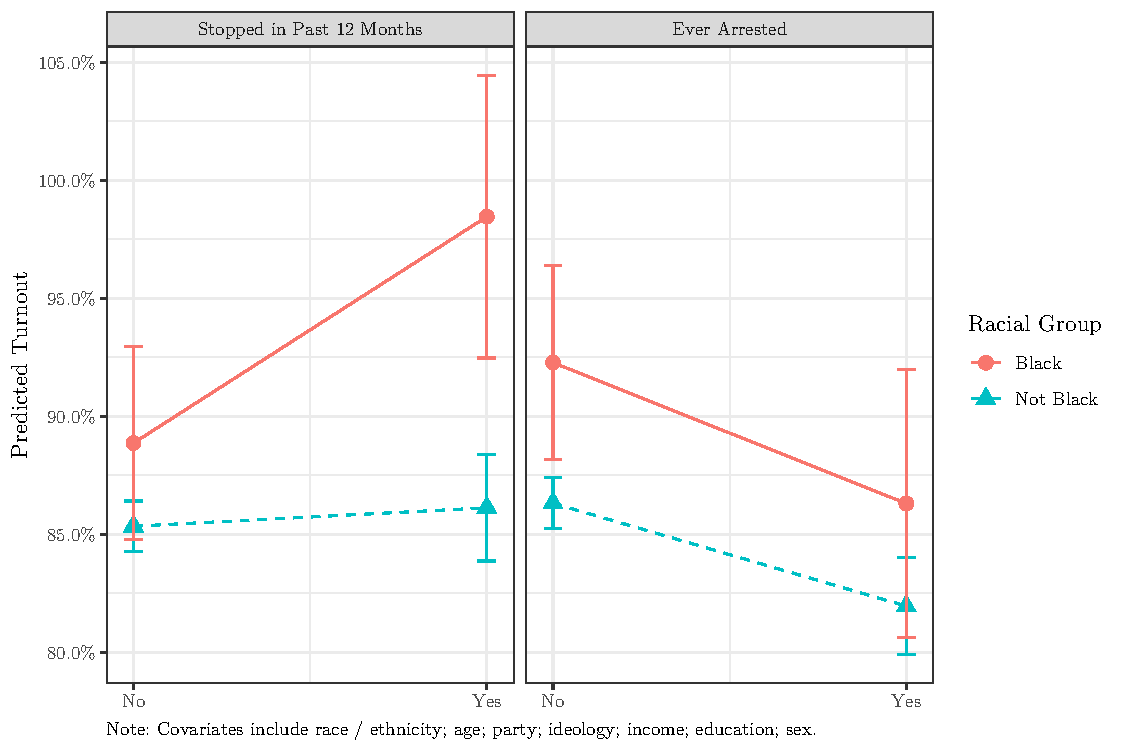
\includegraphics{draft_paper_files/figure-latex/anes-cross-1} 

}

\caption{\label{fig:anes}Predicted Turnout, 2020}\label{fig:anes-cross}
\end{figure}

Figure \ref{fig:anes} demonstrates that Black voters who were stopped by the police, or had a family member stopped by the police, were substantially more likely to vote in 2020 than Black individuals with neither direct nor proximal contact with a police stop (\emph{p} = 0.004). The same was not true for non-Black respondents, for whom contact with a police stop was not statistically associated with turnout in 2020 (\emph{p} = 0.07). Importantly, this effect is not a remnant of a white--nonwhite divide. As we show in the SI, police stops were not differently related to turnout for Latinos than for non-Latinos; nor did they impact turnout differently for Asians than for non-Asians. The ANES results point, then, to the fact that police stops are uniquely associated with higher turnout for Black respondents.

The second panel of Figure \ref{fig:anes} shows that, as expected, respondents who had been arrested at some point turned out at lower rates, after controlling for relevant characteristics. Importantly, the interaction between arrest status and the respondent's race was not statistically significant. In other words, although police stops seem to be uniquely mobilizing for Black Americans, we fail to uncover evidence that arrests differentially structured subsequent Black and non-Black turnout.

It is worth re-establishing that cross-sectional results cannot establish causality. It is possible that Black respondents who had been stopped by the police (or had family members who experienced a stop) differed from non-Black respondents with such contact in ways that cannot be captured by the survey data. However, our findings are consistent with a causal story that police stops are uniquely mobilizing for Black Americans---but this is not the case for higher-level contact, such as arrests.

\hypertarget{discussion}{%
\section*{Discussion}\label{discussion}}
\addcontentsline{toc}{section}{Discussion}

While existing sociological and political science literature has examined the rise and collateral consequences of criminalization on political socialization, no study has investigated the causal relationship between ticketing and voter turnout using individual-level administrative data.

Given how widespread police stops are and their relationship to racial injustice, their political implications demand close study. Accordingly, we investigate this question using two different data sources and analytic strategies. What we find complicates our understanding of how lower-level police contact affects political participation. In the analysis of Hillsborough County police stops, we find that stops reduce the voter turnout of non-Black voters, with a smaller negative effect for Black voters. On the other hand, the descriptive analysis of national survey data indicates that police contact is associated with \emph{higher} turnout for Black Americans, and \emph{unrelated} to turnout for others. Despite this incongruence, both analyses indicate that police stops have different participatory effects for Black individuals than for others. In this sense, our results point in the same direction. We conclude that the political consequences of police stops are unique for Black Americans---and that they are less demobilizing for Black Americans than others. Additionally, as \protect\hyperlink{ref-Walker2020a}{Walker} (\protect\hyperlink{ref-Walker2020a}{2020b}) suggests, ticketed Black individuals may be politically mobilized for activities other than voting not observed in this study, such as contacting elected representatives or volunteering for campaigns. To that end, it is also worth noting that our causal analysis tests the effect of personal police contact rather than proximal contact, which was the focus of \protect\hyperlink{ref-Walker2020a}{Walker} (\protect\hyperlink{ref-Walker2020a}{2020b})---it could be the case that mobilizing effects of low-level police contact come from proximal exposure rather than personal.

Our findings have several implications for political science scholarship. While existing literature suggests that the most disruptive forms of criminal legal contact (i.e.~criminal convictions and incarceration) consistently discourage voting (\protect\hyperlink{ref-Lerman2014}{Lerman and Weaver 2014}; \protect\hyperlink{ref-Burch2011}{Burch 2011}; \protect\hyperlink{ref-White2019a}{White 2019b}), research regarding police stops has produced more mixed results (\protect\hyperlink{ref-Laniyonu2019}{Laniyonu 2019}). We extend this theory to police ticketing, the most common form of police contact in America, and find that police traffic stops generally reduce turnout. For Black voters, however, our findings suggest that traffic stops are less demobilizing, a sharp contrast with existing scholarship wherein more disruptive forms of criminalization discourage Black voters more than non-Black voters. Particularly following the rise of the Black Lives Matter movement in 2013, our findings constitute new evidence in support of our theory that ticketing is distinct from other forms of criminal legal contact and therefore catalyzes different political behaviors among Black voters, who are disproportionately affected by both ticketing and criminalization in general.

In this sense, our analysis could be consistent with a political contestation of criminal legal policy, a phenomenon that aligns with dozens of recent campaigns to reform local fines and fees practices (or abolish them entirely).\footnote{See \url{https://finesandfeesjusticecenter.org/clearinghouse}.} We know that increased fines and fees result from political economy (i.e.~austerity at the federal level), but our analysis suggests that this could be a ``two way street'' wherein people who are harmed by policing practices can be politically socialized into resistance.

\textbf{Limitations}: In our analysis of Hillsborough County voters, we do not look at people who were not registered to vote in 2018. Because we cannot tell whether unregistered individuals who were stopped in Hillsborough County were unregistered because they were \emph{ineligible} to do so (by virtue of living in a different county or being a non-citizen, for instance) or chose to eschew electoral politics, our analysis is necessarily limited to individuals who were registered to vote. This likely makes our results conservative: we cannot capture the lost participation of individuals who would have registered and voted if they were not stopped by the police.

\textbf{Future research}: This work looks at the difference between the political behavior of Black and non-Black Americans. Future work should explore variation \emph{within} the Black community. When is this sort of contact mobilizing? For whom? Can organizers build on this potential for broad-based political action? We were unable to test whether what we observed was simply \emph{decreased} demobilization, or whether some subgroups of the Black population were mobilized while others were demobilized. Put differently: it could be the case that ticketing is demobilizing for most voters of all races, but that a subset of the Black population is affirmatively mobilized, leading to lower group-level demobilization. Scholars should also investigate the interactive effects of criminal legal contact, asking whether police stops result in different political behavior for formerly incarcerated individuals than individuals with no other contact with the system.

Finally, we are sensitive to the fact that although administrative data provides real-world evidence of actual behavior, such an approach limits our ability to understand the causal mechanisms in play. This means that although we demonstrate that police stops are demobilizing, future work must further investigate how stops are interpreted by individuals and translated into political behavior.

Although we have contributed new evidence suggesting that police stops and related exploitative ticketing practices may not demobilize Black voters to the same extent as non-Black voters, we emphasize that this finding does not redeem or justify such police practices. Black Americans already suffer from disproportionate police contact and the racial wealth gap, and racist revenue-motivated ticketing only increases the burden on Black communities nationwide. Policymakers should work to ensure that Black Americans no longer have to struggle to enjoy the same political power as whites---to that end, the current trend of voting rights restriction policies across the country is especially pernicious. Even if some Black Americans understand the ballot box as one tool they can use to limit the state's power to exploit and harm them, policymakers should still feel an obligation to support voting rights protections and stop disproportionate ticketing in Black communities.

\newpage

\hypertarget{references}{%
\section*{References}\label{references}}
\addcontentsline{toc}{section}{References}

\hypertarget{refs}{}
\begin{CSLReferences}{1}{0}
\leavevmode\hypertarget{ref-Ang2021}{}%
Ang, Desmond, Panka Bencsik, Jesse Bruhn, and Ellora Derenoncourt. 2021. {``Police {Violence Reduces Civilian Cooperation} and {Engagement} with {Law Enforcement}.''} \emph{Working Paper.}, September.

\leavevmode\hypertarget{ref-Baumgartner2018}{}%
Baumgartner, Frank R, Derek A Epp, and Kelsey Shoub. 2018. \emph{Suspect Citizens: What 20 Million Traffic Stops Tell Us about Policing and Race}.

\leavevmode\hypertarget{ref-Bell2017}{}%
Bell, Monica C. 2017. {``Police {Reform} and the {Dismantling} of {Legal Estrangement}.''} \emph{The Yale Law Journal} 126 (7): 2054--150.

\leavevmode\hypertarget{ref-Brayne2014}{}%
Brayne, Sarah. 2014. {``Surveillance and {System Avoidance}: {Criminal Justice Contact} and {Institutional Attachment}.''} \emph{American Sociological Review} 79 (3): 367--91. \url{https://doi.org/10.1177/0003122414530398}.

\leavevmode\hypertarget{ref-Burch2011}{}%
Burch, Traci R. 2011. {``Turnout and {Party Registration} Among {Criminal Offenders} in the 2008 {General Election}.''} \emph{Law \& Society Review} 45 (3): 699--730. \url{https://doi.org/10.1111/j.1540-5893.2011.00448.x}.

\leavevmode\hypertarget{ref-Burch2014}{}%
---------. 2014. {``Effects of {Imprisonment} and {Community Supervision} on {Neighborhood Political Participation} in {North Carolina}.''} \emph{The ANNALS of the American Academy of Political and Social Science} 651 (1): 184--201. \url{https://doi.org/10.1177/0002716213503093}.

\leavevmode\hypertarget{ref-CarpenterII2019}{}%
Carpenter II, Dick M, Kyle Sweetland, and Jennifer McDonald. 2019. {``The {Price} of {Taxation} by {Citation}: {Case Studies} of {Three Georgia Cities That Rely Heavily} on {Fines} and {Fees}.''} {Institute for Justice}.

\leavevmode\hypertarget{ref-Desmond2016}{}%
Desmond, Matthew, Andrew V. Papachristos, and David S. Kirk. 2016. {``Police {Violence} and {Citizen Crime Reporting} in the {Black Community}.''} \emph{American Sociological Review} 81 (5): 857--76. \url{https://doi.org/10.1177/0003122416663494}.

\leavevmode\hypertarget{ref-Desmond2020}{}%
---------. 2020. {``Evidence of the {Effect} of {Police Violence} on {Citizen Crime Reporting}.''} \emph{American Sociological Review} 85 (1): 184--90. \url{https://doi.org/10.1177/0003122419895979}.

\leavevmode\hypertarget{ref-Epp2014}{}%
Epp, Charles R., Steven Maynard-Moody, and Donald P. Haider-Markel. 2014. \emph{Pulled {Over}}. {The University of Chicago Press}.

\leavevmode\hypertarget{ref-Gerber2015}{}%
Gerber, Alan S., Gregory A. Huber, Marc Meredith, Daniel R. Biggers, and David J. Hendry. 2015. {``Can {Incarcerated Felons Be} ({Re})integrated into the {Political System}? {Results} from a {Field Experiment}.''} \emph{American Journal of Political Science} 59 (4): 912--26. \url{https://doi.org/10.1111/ajps.12166}.

\leavevmode\hypertarget{ref-Gerber2017}{}%
---------. 2017. {``Does {Incarceration Reduce Voting}? {Evidence} about the {Political Consequences} of {Spending Time} in {Prison}.''} \emph{The Journal of Politics} 79 (4): 1130--46. \url{https://doi.org/10.1086/692670}.

\leavevmode\hypertarget{ref-Harrell2020}{}%
Harrell, Erika, and Elizabeth Davis. 2020. {``Contacts {Between Police} and the {Public}, 2018 - {Statistical Tables}.''} {Bureau of Justice Statistics}.

\leavevmode\hypertarget{ref-Harris2017}{}%
Harris, Alexes, Beth Huebner, Karin Martin, Mary Pattillo, Becky Pettit, Sarah Shannon, Bryan Sykes, Chris Uggen, and April Fernandes. 2017. {``Monetary {Sanctions} in the {Criminal Justice System}.''}

\leavevmode\hypertarget{ref-Harris2020}{}%
Harris, Allison P., Elliott Ash, and Jeffrey Fagan. 2020. {``Fiscal {Pressures} and {Discriminatory Policing}: {Evidence} from {Traffic Stops} in {Missouri}.''} \emph{Journal of Race, Ethnicity, and Politics} 5 (3): 450--80. \url{https://doi.org/10.1017/rep.2020.10}.

\leavevmode\hypertarget{ref-Imai2020}{}%
Imai, Kosuke, In Song Kim, and Erik Wang. 2020. {``Matching {Methods} for {Causal Inference} with {Time-Series Cross-Sectional Data}.''} \emph{Working Paper}. \url{https://doi.org/Matching\%20Methods\%20for\%20Causal\%20Inference\%20with\%20Time-Series\%20Cross-Sectional\%20Data}.

\leavevmode\hypertarget{ref-Jones2019}{}%
Jones, Alexi, and Wendy Sawyer. 2019. {``Arrest, Release, Repeat: {How} Police and Jails Are Misused to Respond to Social Problems.''} {Prison Policy Initiative}.

\leavevmode\hypertarget{ref-Justice2014}{}%
Justice, Benjamin, and Tracey L. Meares. 2014. {``How the {Criminal Justice System Educates Citizens}.''} \emph{The ANNALS of the American Academy of Political and Social Science} 651 (1): 159--77. \url{https://doi.org/10.1177/0002716213502929}.

\leavevmode\hypertarget{ref-Laniyonu2019}{}%
Laniyonu, Ayobami. 2019. {``The {Political Consequences} of {Policing}: {Evidence} from {New York City}.''} \emph{Political Behavior} 41 (2): 527--58. \url{https://doi.org/10.1007/s11109-018-9461-9}.

\leavevmode\hypertarget{ref-Lee2015}{}%
Lee, Hedwig, Tyler McCormick, Margaret T. Hicken, and Christopher Wildeman. 2015. {``Racial {Inequalities} in {Connectedness} to {Imprisoned Individuals} in the {United States}.''} \emph{Du Bois Review: Social Science Research on Race} 12 (2): 269--82. \url{https://doi.org/10.1017/S1742058X15000065}.

\leavevmode\hypertarget{ref-Lee2014}{}%
Lee, Hedwig, Lauren C. Porter, and Megan Comfort. 2014. {``Consequences of {Family Member Incarceration}: {Impacts} on {Civic Participation} and {Perceptions} of the {Legitimacy} and {Fairness} of {Government}.''} \emph{The ANNALS of the American Academy of Political and Social Science} 651 (1): 44--73. \url{https://doi.org/10.1177/0002716213502920}.

\leavevmode\hypertarget{ref-Lerman2014}{}%
Lerman, Amy E., and Vesla M. Weaver. 2014. \emph{Arresting Citizenship: The Democratic Consequences of {American} Crime Control}. Chicago Studies in {American} Politics. {Chicago ; London}: {The University of Chicago Press}.

\leavevmode\hypertarget{ref-Levenson2021}{}%
Levenson, Michael. 2021. {``Pulled {Over}: {What} to {Know About Deadly Police Traffic Stops}.''} \emph{The New York Times}, October.

\leavevmode\hypertarget{ref-Lundberg2021}{}%
Lundberg, Ian, Rebecca Johnson, and Brandon M. Stewart. 2021. {``What {Is Your Estimand}? {Defining} the {Target Quantity Connects Statistical Evidence} to {Theory}.''} \emph{American Sociological Review} 86 (3): 532--65. \url{https://doi.org/10.1177/00031224211004187}.

\leavevmode\hypertarget{ref-McCoy2015}{}%
McCoy, Terrence. 2015. {``Ferguson Shows How a Police Force Can Turn into a Plundering {`Collection Agency'}.''} \emph{Washington Post}, March.

\leavevmode\hypertarget{ref-Meares2017}{}%
Meares, Tracey. 2017. {``Policing and {Procedural Justice}: {Shaping Citizens}' {Identities} to {Increase Democratic Participation}.''} \emph{Northwestern University Law Review} 111 (6): 1525--36.

\leavevmode\hypertarget{ref-Meredith2014}{}%
Meredith, Marc, and Michael Morse. 2014. {``Do {Voting Rights Notification Laws Increase Ex-Felon Turnout}?''} \emph{The ANNALS of the American Academy of Political and Social Science} 651 (1): 220--49. \url{https://doi.org/10.1177/0002716213502931}.

\leavevmode\hypertarget{ref-Meredith2015}{}%
---------. 2015. {``The {Politics} of the {Restoration} of {Ex-Felon Voting Rights}: {The Case} of {Iowa}.''} \emph{Quarterly Journal of Political Science} 10 (1): 41--100. \url{https://doi.org/10.1561/100.00013026}.

\leavevmode\hypertarget{ref-Morris2020}{}%
Morris, Kevin. 2020. {``Neighborhoods and {Felony Disenfranchisement}: {The Case} of {New York City}.''} \emph{Urban Affairs Review}, May, 1078087420921522. \url{https://doi.org/10.1177/1078087420921522}.

\leavevmode\hypertarget{ref-Morris2021a}{}%
---------. 2021a. {``Welcome {Home}{{Now Vote}}! {Voting Rights Restoration} and {Postsupervision Participation}.''} \emph{Social Science Quarterly} 102 (1): 140--53. \url{https://doi.org/10.1111/ssqu.12901}.

\leavevmode\hypertarget{ref-Morris2021}{}%
---------. 2021b. {``Turnout and {Amendment Four}: {Mobilizing Eligible Voters Close} to {Formerly Incarcerated Floridians}.''} \emph{American Political Science Review}, April, 1--16. \url{https://doi.org/10.1017/S0003055421000253}.

\leavevmode\hypertarget{ref-Nyhan2017}{}%
Nyhan, Brendan, Christopher Skovron, and Rocío Titiunik. 2017. {``Differential {Registration Bias} in {Voter File Data}: {A Sensitivity Analysis Approach}.''} \emph{American Journal of Political Science} 61 (3): 744--60. \url{https://doi.org/10.1111/ajps.12288}.

\leavevmode\hypertarget{ref-Pacewicz2020}{}%
Pacewicz, Josh, and John N. Robinson III. 2020. {``Pocketbook Policing: {How} Race Shapes Municipal Reliance on Punitive Fines and Fees in the {Chicago} Suburbs.''} \emph{Socio-Economic Review}, no. mwaa029 (October). \url{https://doi.org/10.1093/ser/mwaa029}.

\leavevmode\hypertarget{ref-Remster2018a}{}%
Remster, Brianna, and Rory Kramer. 2018. {``Race, {Space}, and {Surveillance}: {Understanding} the {Relationship} Between {Criminal Justice Contact} and {Institutional Involvement}.''} \emph{Socius} 4 (January). \url{https://doi.org/10.1177/2378023118761434}.

\leavevmode\hypertarget{ref-Sances2017}{}%
Sances, Michael W., and Hye Young You. 2017. {``Who {Pays} for {Government}? {Descriptive Representation} and {Exploitative Revenue Sources}.''} \emph{The Journal of Politics} 79 (3): 1090--94. \url{https://doi.org/10.1086/691354}.

\leavevmode\hypertarget{ref-Sanders2017}{}%
Sanders, Topher, and Benjamin Conarck. 2017. {``Florida {Police Issue Hundreds} of {Bad Pedestrian Tickets Every Year Because They Don}'t {Seem} to {Know} the {Law}.''} \emph{ProPublica}, December.

\leavevmode\hypertarget{ref-Sekhon2011}{}%
Sekhon, Jasjeet S. 2011. {``Multivariate and {Propensity Score Matching Software} with {Automated Balance Optimization}: {The Matching} Package for {R}.''} \emph{Journal of Statistical Software} 42 (7): 1--52. \url{https://doi.org/10.18637/jss.v042.i07}.

\leavevmode\hypertarget{ref-Shaer2019}{}%
Shaer, Matthew. 2019. {``How {Cities Make Money} by {Fining} the {Poor}.''} \emph{The New York Times}, January.

\leavevmode\hypertarget{ref-Singla2020}{}%
Singla, Akheil, Charlotte Kirschner, and Samuel B. Stone. 2020. {``Race, {Representation}, and {Revenue}: {Reliance} on {Fines} and {Forfeitures} in {City Governments}.''} \emph{Urban Affairs Review} 56 (4): 1132--67. \url{https://doi.org/10.1177/1078087419834632}.

\leavevmode\hypertarget{ref-Soss2017}{}%
Soss, Joe, and Vesla Weaver. 2017. {``Police {Are Our Government}: {Politics}, {Political Science}, and the {Policing} of {Race}{{Class Subjugated Communities}}.''} \emph{Annual Review of Political Science} 20 (1): 565--91. \url{https://doi.org/10.1146/annurev-polisci-060415-093825}.

\leavevmode\hypertarget{ref-Stuart2016}{}%
Stuart, Forrest. 2016. {``Becoming {`{Copwise}'}: {Policing}, {Culture}, and the {Collateral Consequences} of {Street-Level Criminalization}.''} \emph{Law \& Society Review} 50 (2): 279--313. \url{https://doi.org/10.1111/lasr.12201}.

\leavevmode\hypertarget{ref-Tyler2014}{}%
Tyler, Tom R., Jeffrey Fagan, and Amanda Geller. 2014. {``Street {Stops} and {Police Legitimacy}: {Teachable Moments} in {Young Urban Men}'s {Legal Socialization}.''} \emph{Journal of Empirical Legal Studies} 11 (4): 751--85. \url{https://doi.org/10.1111/jels.12055}.

\leavevmode\hypertarget{ref-Uggen2002}{}%
Uggen, Christopher, and Jeff Manza. 2002. {``Democratic {Contraction}? {Political Consequences} of {Felon Disenfranchisement} in the {United States}.''} \emph{American Sociological Review} 67 (6): 777--803. \url{https://doi.org/10.2307/3088970}.

\leavevmode\hypertarget{ref-UnitedStatesDepartmentofJusticeCivilRightsDivision2015}{}%
United States Department of Justice Civil Rights Division. 2015. {``Investigation of the {Ferguson Police Department}.''}

\leavevmode\hypertarget{ref-Walker2014}{}%
Walker, Hannah L. 2014. {``Extending the {Effects} of the {Carceral State}: {Proximal Contact}, {Political Participation}, and {Race}.''} \emph{Political Research Quarterly}, July. \url{https://doi.org/10.1177/1065912914542522}.

\leavevmode\hypertarget{ref-Walker2020}{}%
---------. 2020a. \emph{Mobilized by Injustice: Criminal Justice Contact, Political Participation, and Race}. {NewYork}: {Oxford University Press 2020}.

\leavevmode\hypertarget{ref-Walker2020a}{}%
---------. 2020b. {``Targeted: {The Mobilizing Effect} of {Perceptions} of {Unfair Policing Practices}.''} \emph{The Journal of Politics} 82 (1): 119--34. \url{https://doi.org/10.1086/705684}.

\leavevmode\hypertarget{ref-Weaver2010}{}%
Weaver, Vesla M., and Amy E. Lerman. 2010. {``Political {Consequences} of the {Carceral State}.''} \emph{American Political Science Review} 104 (4): 817--33. \url{https://doi.org/10.1017/S0003055410000456}.

\leavevmode\hypertarget{ref-Weaver2020}{}%
Weaver, Vesla M., Gwen Prowse, and Spencer Piston. 2020. {``Withdrawing and {Drawing In}: {Political Discourse} in {Policed Communities}.''} \emph{Journal of Race, Ethnicity, and Politics} 5 (3): 604--47. \url{https://doi.org/10.1017/rep.2019.50}.

\leavevmode\hypertarget{ref-White2019}{}%
White, Ariel. 2019a. {``Family {Matters}? {Voting Behavior} in {Households} with {Criminal Justice Contact}.''} \emph{American Political Science Review} 113 (2): 607--13. \url{https://doi.org/10.1017/S0003055418000862}.

\leavevmode\hypertarget{ref-White2019a}{}%
---------. 2019b. {``Misdemeanor {Disenfranchisement}? {The Demobilizing Effects} of {Brief Jail Spells} on {Potential Voters}.''} \emph{American Political Science Review} 113 (2): 311--24. \url{https://doi.org/10.1017/S000305541800093X}.

\leavevmode\hypertarget{ref-Zoorob2020}{}%
Zoorob, Michael. 2020. {``Do {Police Brutality Stories Reduce} 911 {Calls}? {Reassessing} an {Important Criminological Finding}.''} \emph{American Sociological Review} 85 (1): 176--83. \url{https://doi.org/10.1177/0003122419895254}.

\end{CSLReferences}

\end{document}
